\documentclass[twoside]{book}

% Packages required by doxygen
\usepackage{fixltx2e}
\usepackage{calc}
\usepackage{doxygen}
\usepackage[export]{adjustbox} % also loads graphicx
\usepackage{graphicx}
\usepackage[utf8]{inputenc}
\usepackage{makeidx}
\usepackage{multicol}
\usepackage{multirow}
\PassOptionsToPackage{warn}{textcomp}
\usepackage{textcomp}
\usepackage[nointegrals]{wasysym}
\usepackage[table]{xcolor}

% NLS support packages
\usepackage[spanish]{babel}
% Font selection
\usepackage[T1]{fontenc}
\usepackage[scaled=.90]{helvet}
\usepackage{courier}
\usepackage{amssymb}
\usepackage{sectsty}
\renewcommand{\familydefault}{\sfdefault}
\allsectionsfont{%
  \fontseries{bc}\selectfont%
  \color{darkgray}%
}
\renewcommand{\DoxyLabelFont}{%
  \fontseries{bc}\selectfont%
  \color{darkgray}%
}
\newcommand{\+}{\discretionary{\mbox{\scriptsize$\hookleftarrow$}}{}{}}

% Page & text layout
\usepackage{geometry}
\geometry{%
  a4paper,%
  top=2.5cm,%
  bottom=2.5cm,%
  left=2.5cm,%
  right=2.5cm%
}
\tolerance=750
\hfuzz=15pt
\hbadness=750
\setlength{\emergencystretch}{15pt}
\setlength{\parindent}{0cm}
\setlength{\parskip}{3ex plus 2ex minus 2ex}
\makeatletter
\renewcommand{\paragraph}{%
  \@startsection{paragraph}{4}{0ex}{-1.0ex}{1.0ex}{%
    \normalfont\normalsize\bfseries\SS@parafont%
  }%
}
\renewcommand{\subparagraph}{%
  \@startsection{subparagraph}{5}{0ex}{-1.0ex}{1.0ex}{%
    \normalfont\normalsize\bfseries\SS@subparafont%
  }%
}
\makeatother

% Headers & footers
\usepackage{fancyhdr}
\pagestyle{fancyplain}
\fancyhead[LE]{\fancyplain{}{\bfseries\thepage}}
\fancyhead[CE]{\fancyplain{}{}}
\fancyhead[RE]{\fancyplain{}{\bfseries\leftmark}}
\fancyhead[LO]{\fancyplain{}{\bfseries\rightmark}}
\fancyhead[CO]{\fancyplain{}{}}
\fancyhead[RO]{\fancyplain{}{\bfseries\thepage}}
\fancyfoot[LE]{\fancyplain{}{}}
\fancyfoot[CE]{\fancyplain{}{}}
\fancyfoot[RE]{\fancyplain{}{\bfseries\scriptsize Generado por Doxygen }}
\fancyfoot[LO]{\fancyplain{}{\bfseries\scriptsize Generado por Doxygen }}
\fancyfoot[CO]{\fancyplain{}{}}
\fancyfoot[RO]{\fancyplain{}{}}
\renewcommand{\footrulewidth}{0.4pt}
\renewcommand{\chaptermark}[1]{%
  \markboth{#1}{}%
}
\renewcommand{\sectionmark}[1]{%
  \markright{\thesection\ #1}%
}

% Indices & bibliography
\usepackage{natbib}
\usepackage[titles]{tocloft}
\setcounter{tocdepth}{3}
\setcounter{secnumdepth}{5}
\makeindex

% Hyperlinks (required, but should be loaded last)
\usepackage{ifpdf}
\ifpdf
  \usepackage[pdftex,pagebackref=true]{hyperref}
\else
  \usepackage[ps2pdf,pagebackref=true]{hyperref}
\fi
\hypersetup{%
  colorlinks=true,%
  linkcolor=blue,%
  citecolor=blue,%
  unicode%
}

% Custom commands
\newcommand{\clearemptydoublepage}{%
  \newpage{\pagestyle{empty}\cleardoublepage}%
}

\usepackage{caption}
\captionsetup{labelsep=space,justification=centering,font={bf},singlelinecheck=off,skip=4pt,position=top}

%===== C O N T E N T S =====

\begin{document}

% Titlepage & ToC
\hypersetup{pageanchor=false,
             bookmarksnumbered=true,
             pdfencoding=unicode
            }
\pagenumbering{alph}
\begin{titlepage}
\vspace*{7cm}
\begin{center}%
{\Large Práctica 2 }\\
\vspace*{1cm}
{\large Generado por Doxygen 1.8.13}\\
\end{center}
\end{titlepage}
\clearemptydoublepage
\pagenumbering{roman}
\tableofcontents
\clearemptydoublepage
\pagenumbering{arabic}
\hypersetup{pageanchor=true}

%--- Begin generated contents ---
\chapter{Rep del T\+DA Cronologia}
\label{repConjunto}
\Hypertarget{repConjunto}
\hypertarget{repConjunto_invConjunto}{}\section{Invariante de la representación}\label{repConjunto_invConjunto}
Para fechas anteriores al año 0 se utilizarán enteros negativos Cada evento debe incluir \# como primer caracter No puede haber dos fechas históricas con el mismo año\hypertarget{repConjunto_faConjunto}{}\section{Función de abstracción}\label{repConjunto_faConjunto}
Un objeto válido {\itshape rep} del T\+DA \hyperlink{classCronologia}{Cronologia} con {\itshape n} tamaño representa al objeto

rep\mbox{[}0\mbox{]}.fecha\+::rep\mbox{[}0\mbox{]}.eventos\mbox{[}0\mbox{]}\#rep\mbox{[}0\mbox{]}.eventos\mbox{[}t-\/1\mbox{]} rep\mbox{[}1\mbox{]}.fecha\+::rep\mbox{[}1\mbox{]}.eventos\mbox{[}0\mbox{]}\#rep\mbox{[}1\mbox{]}.eventos\mbox{[}t-\/1\mbox{]} rep\mbox{[}n-\/1\mbox{]}.fecha\+::rep\mbox{[}n-\/1\mbox{]}.eventos\mbox{[}0\mbox{]}\#rep\mbox{[}n-\/1\mbox{]}.eventos\mbox{[}t-\/1\mbox{]}\hypertarget{repConjunto_invConjunto}{}\section{Invariante de la representación}\label{repConjunto_invConjunto}
Para fechas anteriores al año 0 se utilizarán enteros negativos Cada evento debe incluir \# como primer caracter\hypertarget{repConjunto_faConjunto}{}\section{Función de abstracción}\label{repConjunto_faConjunto}
Un objeto válido {\itshape rep} del T\+DA Fecha\+\_\+\+Historica representa al objeto

rep.\+fecha\+::rep.\+eventos\mbox{[}0\mbox{]}\#rep.\+eventos\mbox{[}n-\/1\mbox{]} 
\chapter{Rep del T\+DA Vector\+Dinamico}
\label{repVectorDinamico}
\Hypertarget{repVectorDinamico}
\hypertarget{repVectorDinamico_invVectorDinamico}{}\section{Invariante de la representación}\label{repVectorDinamico_invVectorDinamico}
Un objeto válido {\itshape v} del T\+DA \hyperlink{classVectorDinamico}{Vector\+Dinamico} debe cumplir
\begin{DoxyItemize}
\item {\ttfamily v.\+nelementos$>$=} 0
\item {\ttfamily v.\+datos} apunta a una zona de memoria con capacidad para albergar {\ttfamily nelementos} valores de tipo {\ttfamily T} 
\end{DoxyItemize}\hypertarget{repVectorDinamico_faVectorDinamico}{}\section{Función de abstracción}\label{repVectorDinamico_faVectorDinamico}
Un objeto vólido {\itshape rep} del T\+DA \hyperlink{classVectorDinamico}{Vector\+Dinamico} representa al vector de tamaño {\itshape n} 

\{v.\+datos\mbox{[}0\mbox{]},v.\+datos\mbox{[}1\mbox{]},...,v.\+datos\mbox{[}v.\+nelementos-\/1\mbox{]}\} 
\chapter{Índice de clases}
\section{Lista de clases}
Lista de las clases, estructuras, uniones e interfaces con una breve descripción\+:\begin{DoxyCompactList}
\item\contentsline{section}{\hyperlink{classDiccionario_1_1const__iterator}{Diccionario$<$ T, U $>$\+::const\+\_\+iterator} \\*T.\+D.\+A \hyperlink{classDiccionario_1_1const__iterator}{const\+\_\+iterator} }{\pageref{classDiccionario_1_1const__iterator}}{}
\item\contentsline{section}{\hyperlink{classDiccionario}{Diccionario$<$ T, U $>$} \\*T.\+D.\+A Diccioanrio }{\pageref{classDiccionario}}{}
\end{DoxyCompactList}

\chapter{Indice de archivos}
\section{Lista de archivos}
Lista de todos los archivos documentados y con descripciones breves\+:\begin{DoxyCompactList}
\item\contentsline{section}{include/\hyperlink{cola_8h}{cola.\+h} \\*Fichero cabecera del T\+DA \hyperlink{classCola}{Cola} }{\pageref{cola_8h}}{}
\item\contentsline{section}{include/{\bfseries cola.\+hpp} }{\pageref{cola_8hpp}}{}
\item\contentsline{section}{include/{\bfseries pila\+\_\+max.\+h} }{\pageref{pila__max_8h}}{}
\item\contentsline{section}{include/\hyperlink{pila__max_8hpp}{pila\+\_\+max.\+hpp} \\*Implementación del T\+DA pila\+\_\+max }{\pageref{pila__max_8hpp}}{}
\end{DoxyCompactList}

\chapter{Documentación de las clases}
\hypertarget{classCronologia}{}\section{Referencia de la Clase Cronologia}
\label{classCronologia}\index{Cronologia@{Cronologia}}


T.\+D.\+A \hyperlink{classCronologia}{Cronologia}.  




{\ttfamily \#include $<$Cronologia.\+h$>$}

\subsection*{Métodos públicos}
\begin{DoxyCompactItemize}
\item 
\hyperlink{classCronologia_ac0026b1919148f6cd6cf4ca4c357771e}{Cronologia} ()
\begin{DoxyCompactList}\small\item\em Constructor por defecto. Crea una cronologia vacía. \end{DoxyCompactList}\item 
\hyperlink{classCronologia_a4de4592918375f3053acee2317dcc711}{Cronologia} (const \hyperlink{classCronologia}{Cronologia} \&original)
\begin{DoxyCompactList}\small\item\em Constructor de copia de la clase. \end{DoxyCompactList}\item 
int \hyperlink{classCronologia_a7eed0b6fa9ddacc5e439e01b00d49fca}{size} () const
\begin{DoxyCompactList}\small\item\em Tamaño de la cronologia. \end{DoxyCompactList}\item 
\hyperlink{classFechaHistorica}{Fecha\+Historica} \hyperlink{classCronologia_a35753d158bfc5abb68c4d28078772bf1}{get\+Fecha} (int i)
\begin{DoxyCompactList}\small\item\em Obtiene la información de una fecha dado su año. \end{DoxyCompactList}\item 
\hyperlink{classFechaHistorica}{Fecha\+Historica} \hyperlink{classCronologia_aaf114dc1d15b4c0032a782a0d8cb2c8c}{get\+Index} (int i)
\begin{DoxyCompactList}\small\item\em Obtiene la información de una fecha segun su indice. \end{DoxyCompactList}\item 
void \hyperlink{classCronologia_a959656bb869865363d796f330fa54ddf}{set\+Fecha} (\hyperlink{classFechaHistorica}{Fecha\+Historica} f)
\begin{DoxyCompactList}\small\item\em Sobreescribe una fecha. \end{DoxyCompactList}\item 
void \hyperlink{classCronologia_a074d231653a08d759ddeb6e5788029f9}{add} (\hyperlink{classFechaHistorica}{Fecha\+Historica} f)
\begin{DoxyCompactList}\small\item\em Añade una nueva fecha a la cronologia. \end{DoxyCompactList}\item 
\hyperlink{classVectorDinamico}{Vector\+Dinamico}$<$ string $>$ \hyperlink{classCronologia_a46137f8c227dc4184dfe9333117108de}{get\+Eventos\+Fecha} (int i)
\begin{DoxyCompactList}\small\item\em Obtiene los eventos que ocurrieron un año. \end{DoxyCompactList}\item 
\hyperlink{classCronologia}{Cronologia} \hyperlink{classCronologia_afd3720750a474b15b082208cf5e557c8}{get\+Eventos\+Entre} (int x, int y)
\begin{DoxyCompactList}\small\item\em Obtiene una nueva cronologia con las fechas cuyos años están entre x e y. \end{DoxyCompactList}\item 
int \hyperlink{classCronologia_a0f9892e61445f393e9c74ba1fc2631c5}{buscar\+Evento} (string s)
\begin{DoxyCompactList}\small\item\em Busca la fecha en la que ocurrio un evento. \end{DoxyCompactList}\item 
\hyperlink{classCronologia}{Cronologia} \& \hyperlink{classCronologia_ac9fddecd2c0a8416d7896d61c74e4dd8}{operator=} (const \hyperlink{classCronologia}{Cronologia} \&c)
\begin{DoxyCompactList}\small\item\em Sobrecarga operador = Permite igualar una cronologia a otra. \end{DoxyCompactList}\item 
\hyperlink{classCronologia}{Cronologia} \hyperlink{classCronologia_a1011faa8363ae7a196301f7693151fad}{operator+} (\hyperlink{classCronologia}{Cronologia} c)
\begin{DoxyCompactList}\small\item\em Sobrecarga operador + Permite sumar dos cronologias. \end{DoxyCompactList}\end{DoxyCompactItemize}
\subsection*{Amigas}
\begin{DoxyCompactItemize}
\item 
ostream \& \hyperlink{classCronologia_a5a590e2ec95cc4489c3de5b03e2cac4c}{operator$<$$<$} (ostream \&os, const \hyperlink{classCronologia}{Cronologia} \&c)
\begin{DoxyCompactList}\small\item\em Sobrecarga del operador $<$$<$. \end{DoxyCompactList}\item 
istream \& \hyperlink{classCronologia_a6fa0f1131309b1cee355b9d8297ea33d}{operator$>$$>$} (istream \&is, \hyperlink{classCronologia}{Cronologia} \&c)
\begin{DoxyCompactList}\small\item\em Sobrecarga del operador $>$$>$. Comprueba si hay saltos de línea vacíos en el fichero para evitar que lo tome como una fecha. \end{DoxyCompactList}\end{DoxyCompactItemize}


\subsection{Descripción detallada}
T.\+D.\+A \hyperlink{classCronologia}{Cronologia}. 

Una instancia {\itshape c} del tipo de datos abstracto {\ttfamily \hyperlink{classCronologia}{Cronologia}} es un objeto con un campo, un {\ttfamily \hyperlink{classVectorDinamico}{Vector\+Dinamico}} de {\ttfamily \hyperlink{classFechaHistorica}{Fecha\+Historica}} El vector contendrá una serie de {\ttfamily \hyperlink{classFechaHistorica}{Fecha\+Historica}} ordenadas por el año de cada una

\begin{DoxyAuthor}{Autor}
Francisco Ruiz Adán 
\end{DoxyAuthor}
\begin{DoxyDate}{Fecha}
17/10/2019 
\end{DoxyDate}


\subsection{Documentación del constructor y destructor}
\mbox{\Hypertarget{classCronologia_ac0026b1919148f6cd6cf4ca4c357771e}\label{classCronologia_ac0026b1919148f6cd6cf4ca4c357771e}} 
\index{Cronologia@{Cronologia}!Cronologia@{Cronologia}}
\index{Cronologia@{Cronologia}!Cronologia@{Cronologia}}
\subsubsection{\texorpdfstring{Cronologia()}{Cronologia()}\hspace{0.1cm}{\footnotesize\ttfamily [1/2]}}
{\footnotesize\ttfamily Cronologia\+::\+Cronologia (\begin{DoxyParamCaption}{ }\end{DoxyParamCaption})}



Constructor por defecto. Crea una cronologia vacía. 

\begin{DoxyReturn}{Devuelve}
Crea una cronologia sin eventos 
\end{DoxyReturn}
\mbox{\Hypertarget{classCronologia_a4de4592918375f3053acee2317dcc711}\label{classCronologia_a4de4592918375f3053acee2317dcc711}} 
\index{Cronologia@{Cronologia}!Cronologia@{Cronologia}}
\index{Cronologia@{Cronologia}!Cronologia@{Cronologia}}
\subsubsection{\texorpdfstring{Cronologia()}{Cronologia()}\hspace{0.1cm}{\footnotesize\ttfamily [2/2]}}
{\footnotesize\ttfamily Cronologia\+::\+Cronologia (\begin{DoxyParamCaption}\item[{const \hyperlink{classCronologia}{Cronologia} \&}]{original }\end{DoxyParamCaption})}



Constructor de copia de la clase. 


\begin{DoxyParams}{Parámetros}
{\em original} & cronologia que se qiere copiar \\
\hline
\end{DoxyParams}
\begin{DoxyReturn}{Devuelve}
crea el objeto con los datos de original 
\end{DoxyReturn}


\subsection{Documentación de las funciones miembro}
\mbox{\Hypertarget{classCronologia_a074d231653a08d759ddeb6e5788029f9}\label{classCronologia_a074d231653a08d759ddeb6e5788029f9}} 
\index{Cronologia@{Cronologia}!add@{add}}
\index{add@{add}!Cronologia@{Cronologia}}
\subsubsection{\texorpdfstring{add()}{add()}}
{\footnotesize\ttfamily void Cronologia\+::add (\begin{DoxyParamCaption}\item[{\hyperlink{classFechaHistorica}{Fecha\+Historica}}]{f }\end{DoxyParamCaption})}



Añade una nueva fecha a la cronologia. 


\begin{DoxyParams}{Parámetros}
{\em f} & nueva fecha a añadir \\
\hline
\end{DoxyParams}
\begin{DoxyPostcond}{Postcondición}
si f ya existe no se añade 
\end{DoxyPostcond}
\mbox{\Hypertarget{classCronologia_a0f9892e61445f393e9c74ba1fc2631c5}\label{classCronologia_a0f9892e61445f393e9c74ba1fc2631c5}} 
\index{Cronologia@{Cronologia}!buscar\+Evento@{buscar\+Evento}}
\index{buscar\+Evento@{buscar\+Evento}!Cronologia@{Cronologia}}
\subsubsection{\texorpdfstring{buscar\+Evento()}{buscarEvento()}}
{\footnotesize\ttfamily int Cronologia\+::buscar\+Evento (\begin{DoxyParamCaption}\item[{string}]{s }\end{DoxyParamCaption})}



Busca la fecha en la que ocurrio un evento. 


\begin{DoxyParams}{Parámetros}
{\em s} & eento cualquiera \\
\hline
\end{DoxyParams}
\begin{DoxyReturn}{Devuelve}
año en el que sucedió el evento o -\/1 si no existe 
\end{DoxyReturn}
\mbox{\Hypertarget{classCronologia_afd3720750a474b15b082208cf5e557c8}\label{classCronologia_afd3720750a474b15b082208cf5e557c8}} 
\index{Cronologia@{Cronologia}!get\+Eventos\+Entre@{get\+Eventos\+Entre}}
\index{get\+Eventos\+Entre@{get\+Eventos\+Entre}!Cronologia@{Cronologia}}
\subsubsection{\texorpdfstring{get\+Eventos\+Entre()}{getEventosEntre()}}
{\footnotesize\ttfamily \hyperlink{classCronologia}{Cronologia} Cronologia\+::get\+Eventos\+Entre (\begin{DoxyParamCaption}\item[{int}]{x,  }\item[{int}]{y }\end{DoxyParamCaption})}



Obtiene una nueva cronologia con las fechas cuyos años están entre x e y. 


\begin{DoxyParams}{Parámetros}
{\em x} & fecha mínima de búsqueda \\
\hline
{\em y} & fecha máxima de búsqueda \\
\hline
\end{DoxyParams}
\begin{DoxyReturn}{Devuelve}
Nueva cronologia con las fechas entre x e y 
\end{DoxyReturn}
\mbox{\Hypertarget{classCronologia_a46137f8c227dc4184dfe9333117108de}\label{classCronologia_a46137f8c227dc4184dfe9333117108de}} 
\index{Cronologia@{Cronologia}!get\+Eventos\+Fecha@{get\+Eventos\+Fecha}}
\index{get\+Eventos\+Fecha@{get\+Eventos\+Fecha}!Cronologia@{Cronologia}}
\subsubsection{\texorpdfstring{get\+Eventos\+Fecha()}{getEventosFecha()}}
{\footnotesize\ttfamily \hyperlink{classVectorDinamico}{Vector\+Dinamico}$<$string$>$ Cronologia\+::get\+Eventos\+Fecha (\begin{DoxyParamCaption}\item[{int}]{i }\end{DoxyParamCaption})}



Obtiene los eventos que ocurrieron un año. 


\begin{DoxyParams}{Parámetros}
{\em i} & años en el que ocurrierons los eventos \\
\hline
\end{DoxyParams}
\begin{DoxyReturn}{Devuelve}
vector$<$string$>$ con los eventos de esa fecha 
\end{DoxyReturn}
\begin{DoxyPostcond}{Postcondición}
si no existe la fecha i devuelve un vector vacío 
\end{DoxyPostcond}
\mbox{\Hypertarget{classCronologia_a35753d158bfc5abb68c4d28078772bf1}\label{classCronologia_a35753d158bfc5abb68c4d28078772bf1}} 
\index{Cronologia@{Cronologia}!get\+Fecha@{get\+Fecha}}
\index{get\+Fecha@{get\+Fecha}!Cronologia@{Cronologia}}
\subsubsection{\texorpdfstring{get\+Fecha()}{getFecha()}}
{\footnotesize\ttfamily \hyperlink{classFechaHistorica}{Fecha\+Historica} Cronologia\+::get\+Fecha (\begin{DoxyParamCaption}\item[{int}]{i }\end{DoxyParamCaption})}



Obtiene la información de una fecha dado su año. 


\begin{DoxyParams}{Parámetros}
{\em i} & año en el que ocurren los eventos \\
\hline
\end{DoxyParams}
\begin{DoxyReturn}{Devuelve}
fecha historica con año {\ttfamily i} Si no se encuentra una fecha con ese año se devuelve una fecha historica vacia con año i 
\end{DoxyReturn}
\mbox{\Hypertarget{classCronologia_aaf114dc1d15b4c0032a782a0d8cb2c8c}\label{classCronologia_aaf114dc1d15b4c0032a782a0d8cb2c8c}} 
\index{Cronologia@{Cronologia}!get\+Index@{get\+Index}}
\index{get\+Index@{get\+Index}!Cronologia@{Cronologia}}
\subsubsection{\texorpdfstring{get\+Index()}{getIndex()}}
{\footnotesize\ttfamily \hyperlink{classFechaHistorica}{Fecha\+Historica} Cronologia\+::get\+Index (\begin{DoxyParamCaption}\item[{int}]{i }\end{DoxyParamCaption})}



Obtiene la información de una fecha segun su indice. 


\begin{DoxyParams}{Parámetros}
{\em i} & indice en el vector \\
\hline
\end{DoxyParams}
\begin{DoxyReturn}{Devuelve}
fecha historica con indice {\ttfamily i} Si no se encuentra una fecha con ese año se devuelve una fecha historica vacia con año i 
\end{DoxyReturn}
\begin{DoxyPrecond}{Precondición}
i debe ser mayor que 0 
\end{DoxyPrecond}
\mbox{\Hypertarget{classCronologia_a1011faa8363ae7a196301f7693151fad}\label{classCronologia_a1011faa8363ae7a196301f7693151fad}} 
\index{Cronologia@{Cronologia}!operator+@{operator+}}
\index{operator+@{operator+}!Cronologia@{Cronologia}}
\subsubsection{\texorpdfstring{operator+()}{operator+()}}
{\footnotesize\ttfamily \hyperlink{classCronologia}{Cronologia} Cronologia\+::operator+ (\begin{DoxyParamCaption}\item[{\hyperlink{classCronologia}{Cronologia}}]{c }\end{DoxyParamCaption})}



Sobrecarga operador + Permite sumar dos cronologias. 


\begin{DoxyParams}{Parámetros}
{\em c} & cronologia a sumar \\
\hline
\end{DoxyParams}
\begin{DoxyReturn}{Devuelve}
nueva cronologia resultado de la suma de esta cronologia y la pasada como parametro 
\end{DoxyReturn}
\mbox{\Hypertarget{classCronologia_ac9fddecd2c0a8416d7896d61c74e4dd8}\label{classCronologia_ac9fddecd2c0a8416d7896d61c74e4dd8}} 
\index{Cronologia@{Cronologia}!operator=@{operator=}}
\index{operator=@{operator=}!Cronologia@{Cronologia}}
\subsubsection{\texorpdfstring{operator=()}{operator=()}}
{\footnotesize\ttfamily \hyperlink{classCronologia}{Cronologia}\& Cronologia\+::operator= (\begin{DoxyParamCaption}\item[{const \hyperlink{classCronologia}{Cronologia} \&}]{c }\end{DoxyParamCaption})}



Sobrecarga operador = Permite igualar una cronologia a otra. 


\begin{DoxyParams}{Parámetros}
{\em c} & cronologia a igualar \\
\hline
\end{DoxyParams}
\mbox{\Hypertarget{classCronologia_a959656bb869865363d796f330fa54ddf}\label{classCronologia_a959656bb869865363d796f330fa54ddf}} 
\index{Cronologia@{Cronologia}!set\+Fecha@{set\+Fecha}}
\index{set\+Fecha@{set\+Fecha}!Cronologia@{Cronologia}}
\subsubsection{\texorpdfstring{set\+Fecha()}{setFecha()}}
{\footnotesize\ttfamily void Cronologia\+::set\+Fecha (\begin{DoxyParamCaption}\item[{\hyperlink{classFechaHistorica}{Fecha\+Historica}}]{f }\end{DoxyParamCaption})}



Sobreescribe una fecha. 


\begin{DoxyParams}{Parámetros}
{\em f} & es la nueva \hyperlink{classFechaHistorica}{Fecha\+Historica} a sobreescribir \\
\hline
\end{DoxyParams}
\begin{DoxyPostcond}{Postcondición}
si f no existe en la cronologia no se hace nada 
\end{DoxyPostcond}
\mbox{\Hypertarget{classCronologia_a7eed0b6fa9ddacc5e439e01b00d49fca}\label{classCronologia_a7eed0b6fa9ddacc5e439e01b00d49fca}} 
\index{Cronologia@{Cronologia}!size@{size}}
\index{size@{size}!Cronologia@{Cronologia}}
\subsubsection{\texorpdfstring{size()}{size()}}
{\footnotesize\ttfamily int Cronologia\+::size (\begin{DoxyParamCaption}{ }\end{DoxyParamCaption}) const}



Tamaño de la cronologia. 

\begin{DoxyReturn}{Devuelve}
Número de fechas guardadas en la cronologia 
\end{DoxyReturn}


\subsection{Documentación de las funciones relacionadas y clases amigas}
\mbox{\Hypertarget{classCronologia_a5a590e2ec95cc4489c3de5b03e2cac4c}\label{classCronologia_a5a590e2ec95cc4489c3de5b03e2cac4c}} 
\index{Cronologia@{Cronologia}!operator$<$$<$@{operator$<$$<$}}
\index{operator$<$$<$@{operator$<$$<$}!Cronologia@{Cronologia}}
\subsubsection{\texorpdfstring{operator$<$$<$}{operator<<}}
{\footnotesize\ttfamily ostream\& operator$<$$<$ (\begin{DoxyParamCaption}\item[{ostream \&}]{os,  }\item[{const \hyperlink{classCronologia}{Cronologia} \&}]{c }\end{DoxyParamCaption})\hspace{0.3cm}{\ttfamily [friend]}}



Sobrecarga del operador $<$$<$. 


\begin{DoxyParams}{Parámetros}
{\em os} & Flujo al que queremos volcar nuestra cronología \\
\hline
{\em c} & Cronología que queremos volcar \\
\hline
\end{DoxyParams}
\mbox{\Hypertarget{classCronologia_a6fa0f1131309b1cee355b9d8297ea33d}\label{classCronologia_a6fa0f1131309b1cee355b9d8297ea33d}} 
\index{Cronologia@{Cronologia}!operator$>$$>$@{operator$>$$>$}}
\index{operator$>$$>$@{operator$>$$>$}!Cronologia@{Cronologia}}
\subsubsection{\texorpdfstring{operator$>$$>$}{operator>>}}
{\footnotesize\ttfamily istream\& operator$>$$>$ (\begin{DoxyParamCaption}\item[{istream \&}]{is,  }\item[{\hyperlink{classCronologia}{Cronologia} \&}]{c }\end{DoxyParamCaption})\hspace{0.3cm}{\ttfamily [friend]}}



Sobrecarga del operador $>$$>$. Comprueba si hay saltos de línea vacíos en el fichero para evitar que lo tome como una fecha. 


\begin{DoxyParams}{Parámetros}
{\em is} & Flujo del que queremos cargar la cronología \\
\hline
{\em c} & Cronología donde queremos cargar el Flujo \\
\hline
\end{DoxyParams}


La documentación para esta clase fue generada a partir del siguiente fichero\+:\begin{DoxyCompactItemize}
\item 
include/Cronologia.\+h\end{DoxyCompactItemize}

\hypertarget{classFechaHistorica}{}\section{Referencia de la Clase Fecha\+Historica}
\label{classFechaHistorica}\index{Fecha\+Historica@{Fecha\+Historica}}


T.\+D.\+A. Fecha Historica.  




{\ttfamily \#include $<$Fecha\+Historica.\+h$>$}

\subsection*{Métodos públicos}
\begin{DoxyCompactItemize}
\item 
\hyperlink{classFechaHistorica_a35baa09e365240e567049a7e33a7c209}{Fecha\+Historica} ()
\begin{DoxyCompactList}\small\item\em Constructor por defecto. \end{DoxyCompactList}\item 
\hyperlink{classFechaHistorica_abf2f8b43afe7baae644fcc8315236eb4}{Fecha\+Historica} (int year)
\begin{DoxyCompactList}\small\item\em Constructor con un parámetro de la clase. El usuario puede crear una fecha indicando solo el año. \end{DoxyCompactList}\item 
\hyperlink{classFechaHistorica_a40a9c133a139d41bf84406e09022feaf}{Fecha\+Historica} (const \hyperlink{classFechaHistorica}{Fecha\+Historica} \&f)
\begin{DoxyCompactList}\small\item\em Constructor copia. \end{DoxyCompactList}\item 
int \hyperlink{classFechaHistorica_acf81e1528a9c7e813626873745cd55d7}{get\+Fecha} () const
\begin{DoxyCompactList}\small\item\em Método de acceso al año de la \hyperlink{classFechaHistorica}{Fecha\+Historica}. \end{DoxyCompactList}\item 
int \hyperlink{classFechaHistorica_aa63596d45eda999d9d65ea4eae22342f}{get\+Num\+Sucesos} () const
\begin{DoxyCompactList}\small\item\em Método de acceso a la cantidad de eventos almacenados en el vector dinámico. \end{DoxyCompactList}\item 
\hyperlink{classVectorDinamico}{Vector\+Dinamico}$<$ string $>$ \hyperlink{classFechaHistorica_a6e2e1ba20212a9d252271b533a259636}{get\+Sucesos} ()
\begin{DoxyCompactList}\small\item\em Método que devuelve los acontecimientos. \end{DoxyCompactList}\item 
void \hyperlink{classFechaHistorica_a82780229e85e6647f59bcf23115d155e}{set\+Year} (int x)
\begin{DoxyCompactList}\small\item\em Modifica el año. \end{DoxyCompactList}\item 
void \hyperlink{classFechaHistorica_a4a6640c33a0662558b9eedbcc15dfa9c}{add\+Suceso} (string suceso)
\begin{DoxyCompactList}\small\item\em Añade un evento. \end{DoxyCompactList}\item 
bool \hyperlink{classFechaHistorica_a4797dd16e39a00d6390138c56974b6d7}{existe\+Suceso} (string suceso) const
\begin{DoxyCompactList}\small\item\em Consulta si existe un evento. \end{DoxyCompactList}\item 
\hyperlink{classFechaHistorica}{Fecha\+Historica} \& \hyperlink{classFechaHistorica_ae7cf51e42c94b39ee8a35840a86bc8e4}{operator=} (const \hyperlink{classFechaHistorica}{Fecha\+Historica} \&nuevo)
\begin{DoxyCompactList}\small\item\em Sobrecarga del operador =. Permite igualar una fecha a otra. \end{DoxyCompactList}\item 
\hyperlink{classFechaHistorica}{Fecha\+Historica} \hyperlink{classFechaHistorica_a6c9e0799d9c70e9ef5e76abe2894f374}{operator+} (\hyperlink{classFechaHistorica}{Fecha\+Historica} f)
\begin{DoxyCompactList}\small\item\em Sobrecarga del operador +. Permite sumar dos fechas. \end{DoxyCompactList}\end{DoxyCompactItemize}
\subsection*{Amigas}
\begin{DoxyCompactItemize}
\item 
ostream \& \hyperlink{classFechaHistorica_ae7ffc75da1b9b42da839968d57c0dc9c}{operator$<$$<$} (ostream \&os, const \hyperlink{classFechaHistorica}{Fecha\+Historica} \&f)
\begin{DoxyCompactList}\small\item\em Sobrecarga del operador $<$$<$. \end{DoxyCompactList}\item 
istream \& \hyperlink{classFechaHistorica_a25a93d162aadd3c52aa1f3d1831e3d75}{operator$>$$>$} (istream \&is, \hyperlink{classFechaHistorica}{Fecha\+Historica} \&f)
\begin{DoxyCompactList}\small\item\em Sobrecarga del operador $>$$>$. Comprueba si hay saltos de línea vacíos en el fichero para evitar que lo tome como una fecha. \end{DoxyCompactList}\end{DoxyCompactItemize}


\subsection{Descripción detallada}
T.\+D.\+A. Fecha Historica. 

Una instancia {\itshape c} del T\+DA {\ttfamily Fecha\+\_\+\+Historica} es un objeto que almacena acontecimientos ocurridos a lo largo de un año. Está compuesto por un valor entero que representa el año y un vector de string para representar los diferentes acontecimientos Lo representamos\+: fecha\+::evento\+::evento...

\begin{DoxyAuthor}{Autor}
Francisco Ruiz Adán 
\end{DoxyAuthor}
\begin{DoxyDate}{Fecha}
17/10/2019 
\end{DoxyDate}


\subsection{Documentación del constructor y destructor}
\mbox{\Hypertarget{classFechaHistorica_a35baa09e365240e567049a7e33a7c209}\label{classFechaHistorica_a35baa09e365240e567049a7e33a7c209}} 
\index{Fecha\+Historica@{Fecha\+Historica}!Fecha\+Historica@{Fecha\+Historica}}
\index{Fecha\+Historica@{Fecha\+Historica}!Fecha\+Historica@{Fecha\+Historica}}
\subsubsection{\texorpdfstring{Fecha\+Historica()}{FechaHistorica()}\hspace{0.1cm}{\footnotesize\ttfamily [1/3]}}
{\footnotesize\ttfamily Fecha\+Historica\+::\+Fecha\+Historica (\begin{DoxyParamCaption}{ }\end{DoxyParamCaption})}



Constructor por defecto. 

\begin{DoxyReturn}{Devuelve}
Crea uuna fecha con año 0 y sin hechos 
\end{DoxyReturn}
\mbox{\Hypertarget{classFechaHistorica_abf2f8b43afe7baae644fcc8315236eb4}\label{classFechaHistorica_abf2f8b43afe7baae644fcc8315236eb4}} 
\index{Fecha\+Historica@{Fecha\+Historica}!Fecha\+Historica@{Fecha\+Historica}}
\index{Fecha\+Historica@{Fecha\+Historica}!Fecha\+Historica@{Fecha\+Historica}}
\subsubsection{\texorpdfstring{Fecha\+Historica()}{FechaHistorica()}\hspace{0.1cm}{\footnotesize\ttfamily [2/3]}}
{\footnotesize\ttfamily Fecha\+Historica\+::\+Fecha\+Historica (\begin{DoxyParamCaption}\item[{int}]{year }\end{DoxyParamCaption})}



Constructor con un parámetro de la clase. El usuario puede crear una fecha indicando solo el año. 


\begin{DoxyParams}{Parámetros}
{\em y} & año del evento a construir \\
\hline
\end{DoxyParams}
\begin{DoxyReturn}{Devuelve}
Crea el evento con los datos de y, el vector de eventos quedará vacío 
\end{DoxyReturn}
\mbox{\Hypertarget{classFechaHistorica_a40a9c133a139d41bf84406e09022feaf}\label{classFechaHistorica_a40a9c133a139d41bf84406e09022feaf}} 
\index{Fecha\+Historica@{Fecha\+Historica}!Fecha\+Historica@{Fecha\+Historica}}
\index{Fecha\+Historica@{Fecha\+Historica}!Fecha\+Historica@{Fecha\+Historica}}
\subsubsection{\texorpdfstring{Fecha\+Historica()}{FechaHistorica()}\hspace{0.1cm}{\footnotesize\ttfamily [3/3]}}
{\footnotesize\ttfamily Fecha\+Historica\+::\+Fecha\+Historica (\begin{DoxyParamCaption}\item[{const \hyperlink{classFechaHistorica}{Fecha\+Historica} \&}]{f }\end{DoxyParamCaption})}



Constructor copia. 


\begin{DoxyParams}{Parámetros}
{\em f} & \hyperlink{classFechaHistorica}{Fecha\+Historica} que se quiere copiar \\
\hline
\end{DoxyParams}
\begin{DoxyReturn}{Devuelve}
Crea el objeto con los datos de f 
\end{DoxyReturn}


\subsection{Documentación de las funciones miembro}
\mbox{\Hypertarget{classFechaHistorica_a4a6640c33a0662558b9eedbcc15dfa9c}\label{classFechaHistorica_a4a6640c33a0662558b9eedbcc15dfa9c}} 
\index{Fecha\+Historica@{Fecha\+Historica}!add\+Suceso@{add\+Suceso}}
\index{add\+Suceso@{add\+Suceso}!Fecha\+Historica@{Fecha\+Historica}}
\subsubsection{\texorpdfstring{add\+Suceso()}{addSuceso()}}
{\footnotesize\ttfamily void Fecha\+Historica\+::add\+Suceso (\begin{DoxyParamCaption}\item[{string}]{suceso }\end{DoxyParamCaption})}



Añade un evento. 


\begin{DoxyParams}{Parámetros}
{\em suceso} & string con evento a añadir \\
\hline
\end{DoxyParams}
\mbox{\Hypertarget{classFechaHistorica_a4797dd16e39a00d6390138c56974b6d7}\label{classFechaHistorica_a4797dd16e39a00d6390138c56974b6d7}} 
\index{Fecha\+Historica@{Fecha\+Historica}!existe\+Suceso@{existe\+Suceso}}
\index{existe\+Suceso@{existe\+Suceso}!Fecha\+Historica@{Fecha\+Historica}}
\subsubsection{\texorpdfstring{existe\+Suceso()}{existeSuceso()}}
{\footnotesize\ttfamily bool Fecha\+Historica\+::existe\+Suceso (\begin{DoxyParamCaption}\item[{string}]{suceso }\end{DoxyParamCaption}) const}



Consulta si existe un evento. 


\begin{DoxyParams}{Parámetros}
{\em s} & evento que se desea saber si está \\
\hline
\end{DoxyParams}
\begin{DoxyReturn}{Devuelve}
bool con verdadero si está, false si no se existe 
\end{DoxyReturn}
\mbox{\Hypertarget{classFechaHistorica_acf81e1528a9c7e813626873745cd55d7}\label{classFechaHistorica_acf81e1528a9c7e813626873745cd55d7}} 
\index{Fecha\+Historica@{Fecha\+Historica}!get\+Fecha@{get\+Fecha}}
\index{get\+Fecha@{get\+Fecha}!Fecha\+Historica@{Fecha\+Historica}}
\subsubsection{\texorpdfstring{get\+Fecha()}{getFecha()}}
{\footnotesize\ttfamily int Fecha\+Historica\+::get\+Fecha (\begin{DoxyParamCaption}{ }\end{DoxyParamCaption}) const}



Método de acceso al año de la \hyperlink{classFechaHistorica}{Fecha\+Historica}. 

\begin{DoxyReturn}{Devuelve}
int con el valor del campo year 
\end{DoxyReturn}
\mbox{\Hypertarget{classFechaHistorica_aa63596d45eda999d9d65ea4eae22342f}\label{classFechaHistorica_aa63596d45eda999d9d65ea4eae22342f}} 
\index{Fecha\+Historica@{Fecha\+Historica}!get\+Num\+Sucesos@{get\+Num\+Sucesos}}
\index{get\+Num\+Sucesos@{get\+Num\+Sucesos}!Fecha\+Historica@{Fecha\+Historica}}
\subsubsection{\texorpdfstring{get\+Num\+Sucesos()}{getNumSucesos()}}
{\footnotesize\ttfamily int Fecha\+Historica\+::get\+Num\+Sucesos (\begin{DoxyParamCaption}{ }\end{DoxyParamCaption}) const}



Método de acceso a la cantidad de eventos almacenados en el vector dinámico. 

\begin{DoxyReturn}{Devuelve}
int con el número de eventos almacenados en el vector dinámico 
\end{DoxyReturn}
\mbox{\Hypertarget{classFechaHistorica_a6e2e1ba20212a9d252271b533a259636}\label{classFechaHistorica_a6e2e1ba20212a9d252271b533a259636}} 
\index{Fecha\+Historica@{Fecha\+Historica}!get\+Sucesos@{get\+Sucesos}}
\index{get\+Sucesos@{get\+Sucesos}!Fecha\+Historica@{Fecha\+Historica}}
\subsubsection{\texorpdfstring{get\+Sucesos()}{getSucesos()}}
{\footnotesize\ttfamily \hyperlink{classVectorDinamico}{Vector\+Dinamico}$<$string$>$ Fecha\+Historica\+::get\+Sucesos (\begin{DoxyParamCaption}{ }\end{DoxyParamCaption})}



Método que devuelve los acontecimientos. 

\begin{DoxyReturn}{Devuelve}
vector$<$string$>$ con los hechos 
\end{DoxyReturn}
\mbox{\Hypertarget{classFechaHistorica_a6c9e0799d9c70e9ef5e76abe2894f374}\label{classFechaHistorica_a6c9e0799d9c70e9ef5e76abe2894f374}} 
\index{Fecha\+Historica@{Fecha\+Historica}!operator+@{operator+}}
\index{operator+@{operator+}!Fecha\+Historica@{Fecha\+Historica}}
\subsubsection{\texorpdfstring{operator+()}{operator+()}}
{\footnotesize\ttfamily \hyperlink{classFechaHistorica}{Fecha\+Historica} Fecha\+Historica\+::operator+ (\begin{DoxyParamCaption}\item[{\hyperlink{classFechaHistorica}{Fecha\+Historica}}]{f }\end{DoxyParamCaption})}



Sobrecarga del operador +. Permite sumar dos fechas. 


\begin{DoxyParams}{Parámetros}
{\em f} & \hyperlink{classFechaHistorica}{Fecha\+Historica} que se quiere sumar \\
\hline
\end{DoxyParams}
\mbox{\Hypertarget{classFechaHistorica_ae7cf51e42c94b39ee8a35840a86bc8e4}\label{classFechaHistorica_ae7cf51e42c94b39ee8a35840a86bc8e4}} 
\index{Fecha\+Historica@{Fecha\+Historica}!operator=@{operator=}}
\index{operator=@{operator=}!Fecha\+Historica@{Fecha\+Historica}}
\subsubsection{\texorpdfstring{operator=()}{operator=()}}
{\footnotesize\ttfamily \hyperlink{classFechaHistorica}{Fecha\+Historica}\& Fecha\+Historica\+::operator= (\begin{DoxyParamCaption}\item[{const \hyperlink{classFechaHistorica}{Fecha\+Historica} \&}]{nuevo }\end{DoxyParamCaption})}



Sobrecarga del operador =. Permite igualar una fecha a otra. 


\begin{DoxyParams}{Parámetros}
{\em nuevo} & \hyperlink{classFechaHistorica}{Fecha\+Historica} a la que se quiere igualar \\
\hline
\end{DoxyParams}
\mbox{\Hypertarget{classFechaHistorica_a82780229e85e6647f59bcf23115d155e}\label{classFechaHistorica_a82780229e85e6647f59bcf23115d155e}} 
\index{Fecha\+Historica@{Fecha\+Historica}!set\+Year@{set\+Year}}
\index{set\+Year@{set\+Year}!Fecha\+Historica@{Fecha\+Historica}}
\subsubsection{\texorpdfstring{set\+Year()}{setYear()}}
{\footnotesize\ttfamily void Fecha\+Historica\+::set\+Year (\begin{DoxyParamCaption}\item[{int}]{x }\end{DoxyParamCaption})}



Modifica el año. 


\begin{DoxyParams}{Parámetros}
{\em x} & año de los eventos a construir \\
\hline
\end{DoxyParams}


\subsection{Documentación de las funciones relacionadas y clases amigas}
\mbox{\Hypertarget{classFechaHistorica_ae7ffc75da1b9b42da839968d57c0dc9c}\label{classFechaHistorica_ae7ffc75da1b9b42da839968d57c0dc9c}} 
\index{Fecha\+Historica@{Fecha\+Historica}!operator$<$$<$@{operator$<$$<$}}
\index{operator$<$$<$@{operator$<$$<$}!Fecha\+Historica@{Fecha\+Historica}}
\subsubsection{\texorpdfstring{operator$<$$<$}{operator<<}}
{\footnotesize\ttfamily ostream\& operator$<$$<$ (\begin{DoxyParamCaption}\item[{ostream \&}]{os,  }\item[{const \hyperlink{classFechaHistorica}{Fecha\+Historica} \&}]{f }\end{DoxyParamCaption})\hspace{0.3cm}{\ttfamily [friend]}}



Sobrecarga del operador $<$$<$. 


\begin{DoxyParams}{Parámetros}
{\em os} & Flujo al que queremos volcar nuestra cronología \\
\hline
{\em c} & Cronología que queremos volcar \\
\hline
\end{DoxyParams}
\mbox{\Hypertarget{classFechaHistorica_a25a93d162aadd3c52aa1f3d1831e3d75}\label{classFechaHistorica_a25a93d162aadd3c52aa1f3d1831e3d75}} 
\index{Fecha\+Historica@{Fecha\+Historica}!operator$>$$>$@{operator$>$$>$}}
\index{operator$>$$>$@{operator$>$$>$}!Fecha\+Historica@{Fecha\+Historica}}
\subsubsection{\texorpdfstring{operator$>$$>$}{operator>>}}
{\footnotesize\ttfamily istream\& operator$>$$>$ (\begin{DoxyParamCaption}\item[{istream \&}]{is,  }\item[{\hyperlink{classFechaHistorica}{Fecha\+Historica} \&}]{f }\end{DoxyParamCaption})\hspace{0.3cm}{\ttfamily [friend]}}



Sobrecarga del operador $>$$>$. Comprueba si hay saltos de línea vacíos en el fichero para evitar que lo tome como una fecha. 


\begin{DoxyParams}{Parámetros}
{\em is} & Flujo del que queremos cargar la cronología \\
\hline
{\em c} & Cronología donde queremos cargar el Flujo \\
\hline
\end{DoxyParams}


La documentación para esta clase fue generada a partir del siguiente fichero\+:\begin{DoxyCompactItemize}
\item 
include/\hyperlink{FechaHistorica_8h}{Fecha\+Historica.\+h}\end{DoxyCompactItemize}

\hypertarget{classVectorDinamico}{}\section{Referencia de la plantilla de la Clase Vector\+Dinamico$<$ T $>$}
\label{classVectorDinamico}\index{Vector\+Dinamico$<$ T $>$@{Vector\+Dinamico$<$ T $>$}}


T.\+D.\+A. \hyperlink{classVectorDinamico}{Vector\+Dinamico}.  




{\ttfamily \#include $<$vector\+\_\+dinamico.\+h$>$}

\subsection*{Métodos públicos}
\begin{DoxyCompactItemize}
\item 
\hyperlink{classVectorDinamico_ad1d9b40e76d3ac449e99da4290e08924}{Vector\+Dinamico} (int n=0)
\begin{DoxyCompactList}\small\item\em Constructor por defecto. \end{DoxyCompactList}\item 
\mbox{\Hypertarget{classVectorDinamico_a32117d987800176b81b5b288a15fa80e}\label{classVectorDinamico_a32117d987800176b81b5b288a15fa80e}} 
{\bfseries Vector\+Dinamico} (const \hyperlink{classVectorDinamico}{Vector\+Dinamico}$<$ T $>$ \&original)
\item 
int \hyperlink{classVectorDinamico_a170abdfac52375020f44bc3903f23b65}{size} () const
\begin{DoxyCompactList}\small\item\em Número de componentes del vector. \end{DoxyCompactList}\item 
T \& \hyperlink{classVectorDinamico_a6c4cab2d396b71939c056fb40ba72951}{operator\mbox{[}$\,$\mbox{]}} (int i)
\begin{DoxyCompactList}\small\item\em Acceso a un elemento. \end{DoxyCompactList}\item 
const T \& \hyperlink{classVectorDinamico_ad078d3fb05f126632fd8fe995fae2a74}{operator\mbox{[}$\,$\mbox{]}} (int i) const
\begin{DoxyCompactList}\small\item\em Acceso a un elemento de un vector constante. \end{DoxyCompactList}\item 
void \hyperlink{classVectorDinamico_a9b3fd8907bc3ca9b5bc5775bbb11f867}{resize} (int n)
\begin{DoxyCompactList}\small\item\em Redimensión del vector. \end{DoxyCompactList}\item 
void \hyperlink{classVectorDinamico_a2680351f2cd4feba8825c6f1f04a6392}{push\+\_\+back} (T \&s)
\begin{DoxyCompactList}\small\item\em Añade un elemento al final del vector. \end{DoxyCompactList}\item 
\hyperlink{classVectorDinamico}{Vector\+Dinamico}$<$ T $>$ \& \hyperlink{classVectorDinamico_a94727e698cadc2cf3e8482ce9620df87}{operator=} (const \hyperlink{classVectorDinamico}{Vector\+Dinamico}$<$ T $>$ \&original)
\begin{DoxyCompactList}\small\item\em Sobrecarga del operador de asignacion. \end{DoxyCompactList}\end{DoxyCompactItemize}


\subsection{Descripción detallada}
\subsubsection*{template$<$class T$>$\newline
class Vector\+Dinamico$<$ T $>$}

T.\+D.\+A. \hyperlink{classVectorDinamico}{Vector\+Dinamico}. 

Una instancia {\itshape v} del tipo de datos abstracto {\ttfamily \hyperlink{classVectorDinamico}{Vector\+Dinamico}} sobre el tipo {\ttfamily T} es un array 1-\/dimensional de un determinado tamaño {\itshape n}, que puede crecer y decrecer a petici�n del usuario. Lo podemos representar como

\{v\mbox{[}0\mbox{]},v\mbox{[}1\mbox{]},...,v\mbox{[}n-\/1\mbox{]}\}

donde v\mbox{[}i\mbox{]} es el valor almacenado en la posición i del vector

La eficiencia en espacio es {\itshape O(n)}. 

\subsection{Documentación del constructor y destructor}
\mbox{\Hypertarget{classVectorDinamico_ad1d9b40e76d3ac449e99da4290e08924}\label{classVectorDinamico_ad1d9b40e76d3ac449e99da4290e08924}} 
\index{Vector\+Dinamico@{Vector\+Dinamico}!Vector\+Dinamico@{Vector\+Dinamico}}
\index{Vector\+Dinamico@{Vector\+Dinamico}!Vector\+Dinamico@{Vector\+Dinamico}}
\subsubsection{\texorpdfstring{Vector\+Dinamico()}{VectorDinamico()}}
{\footnotesize\ttfamily template$<$class T $>$ \\
\hyperlink{classVectorDinamico}{Vector\+Dinamico}$<$ T $>$\+::\hyperlink{classVectorDinamico}{Vector\+Dinamico} (\begin{DoxyParamCaption}\item[{int}]{n = {\ttfamily 0} }\end{DoxyParamCaption})}



Constructor por defecto. 


\begin{DoxyParams}{Parámetros}
{\em n} & indica el número de componentes inicial reservados para el vector \\
\hline
\end{DoxyParams}
\begin{DoxyNote}{Nota}
Este constructor también corresponde al de por defecto 
\end{DoxyNote}


\subsection{Documentación de las funciones miembro}
\mbox{\Hypertarget{classVectorDinamico_a94727e698cadc2cf3e8482ce9620df87}\label{classVectorDinamico_a94727e698cadc2cf3e8482ce9620df87}} 
\index{Vector\+Dinamico@{Vector\+Dinamico}!operator=@{operator=}}
\index{operator=@{operator=}!Vector\+Dinamico@{Vector\+Dinamico}}
\subsubsection{\texorpdfstring{operator=()}{operator=()}}
{\footnotesize\ttfamily template$<$class T$>$ \\
\hyperlink{classVectorDinamico}{Vector\+Dinamico}$<$ T $>$ \& \hyperlink{classVectorDinamico}{Vector\+Dinamico}$<$ T $>$\+::operator= (\begin{DoxyParamCaption}\item[{const \hyperlink{classVectorDinamico}{Vector\+Dinamico}$<$ T $>$ \&}]{original }\end{DoxyParamCaption})}



Sobrecarga del operador de asignacion. 


\begin{DoxyParams}{Parámetros}
{\em original} & Vector desde el que se quiere copiar \\
\hline
\end{DoxyParams}
\mbox{\Hypertarget{classVectorDinamico_a6c4cab2d396b71939c056fb40ba72951}\label{classVectorDinamico_a6c4cab2d396b71939c056fb40ba72951}} 
\index{Vector\+Dinamico@{Vector\+Dinamico}!operator\mbox{[}\mbox{]}@{operator[]}}
\index{operator\mbox{[}\mbox{]}@{operator[]}!Vector\+Dinamico@{Vector\+Dinamico}}
\subsubsection{\texorpdfstring{operator[]()}{operator[]()}\hspace{0.1cm}{\footnotesize\ttfamily [1/2]}}
{\footnotesize\ttfamily template$<$class T $>$ \\
T \& \hyperlink{classVectorDinamico}{Vector\+Dinamico}$<$ T $>$\+::operator\mbox{[}$\,$\mbox{]} (\begin{DoxyParamCaption}\item[{int}]{i }\end{DoxyParamCaption})}



Acceso a un elemento. 


\begin{DoxyParams}{Parámetros}
{\em i} & la posición del vector donde está el componente. 0$<$=i$<$\hyperlink{classVectorDinamico_a170abdfac52375020f44bc3903f23b65}{size()} \\
\hline
\end{DoxyParams}
\begin{DoxyReturn}{Devuelve}
La referencia al elemento. Por tanto, se puede usar para almacenar un valor en esa posición. 
\end{DoxyReturn}
\mbox{\Hypertarget{classVectorDinamico_ad078d3fb05f126632fd8fe995fae2a74}\label{classVectorDinamico_ad078d3fb05f126632fd8fe995fae2a74}} 
\index{Vector\+Dinamico@{Vector\+Dinamico}!operator\mbox{[}\mbox{]}@{operator[]}}
\index{operator\mbox{[}\mbox{]}@{operator[]}!Vector\+Dinamico@{Vector\+Dinamico}}
\subsubsection{\texorpdfstring{operator[]()}{operator[]()}\hspace{0.1cm}{\footnotesize\ttfamily [2/2]}}
{\footnotesize\ttfamily template$<$class T $>$ \\
const T \& \hyperlink{classVectorDinamico}{Vector\+Dinamico}$<$ T $>$\+::operator\mbox{[}$\,$\mbox{]} (\begin{DoxyParamCaption}\item[{int}]{i }\end{DoxyParamCaption}) const}



Acceso a un elemento de un vector constante. 


\begin{DoxyParams}{Parámetros}
{\em i} & la posición del vector donde está el componente. 0$<$=i$<$\hyperlink{classVectorDinamico_a170abdfac52375020f44bc3903f23b65}{size()} \\
\hline
\end{DoxyParams}
\begin{DoxyReturn}{Devuelve}
La referencia al elemento. Se supone que el vector no se puede modificar y por tanto es acceso de sólo lectura 
\end{DoxyReturn}
\mbox{\Hypertarget{classVectorDinamico_a2680351f2cd4feba8825c6f1f04a6392}\label{classVectorDinamico_a2680351f2cd4feba8825c6f1f04a6392}} 
\index{Vector\+Dinamico@{Vector\+Dinamico}!push\+\_\+back@{push\+\_\+back}}
\index{push\+\_\+back@{push\+\_\+back}!Vector\+Dinamico@{Vector\+Dinamico}}
\subsubsection{\texorpdfstring{push\+\_\+back()}{push\_back()}}
{\footnotesize\ttfamily template$<$class T$>$ \\
void \hyperlink{classVectorDinamico}{Vector\+Dinamico}$<$ T $>$\+::push\+\_\+back (\begin{DoxyParamCaption}\item[{T \&}]{s }\end{DoxyParamCaption})}



Añade un elemento al final del vector. 


\begin{DoxyParams}{Parámetros}
{\em s} & El nuevo valor a añadir \\
\hline
\end{DoxyParams}
\mbox{\Hypertarget{classVectorDinamico_a9b3fd8907bc3ca9b5bc5775bbb11f867}\label{classVectorDinamico_a9b3fd8907bc3ca9b5bc5775bbb11f867}} 
\index{Vector\+Dinamico@{Vector\+Dinamico}!resize@{resize}}
\index{resize@{resize}!Vector\+Dinamico@{Vector\+Dinamico}}
\subsubsection{\texorpdfstring{resize()}{resize()}}
{\footnotesize\ttfamily template$<$class T $>$ \\
void \hyperlink{classVectorDinamico}{Vector\+Dinamico}$<$ T $>$\+::resize (\begin{DoxyParamCaption}\item[{int}]{n }\end{DoxyParamCaption})}



Redimensión del vector. 


\begin{DoxyParams}{Parámetros}
{\em n} & El nuevo tamaño del vector. n$>$=0 \\
\hline
\end{DoxyParams}
\begin{DoxyPostcond}{Postcondición}
Los valores almacenados antes de la redimensión no se pierden (excepto los que se salen del nuevo rango de índices) 
\end{DoxyPostcond}
\mbox{\Hypertarget{classVectorDinamico_a170abdfac52375020f44bc3903f23b65}\label{classVectorDinamico_a170abdfac52375020f44bc3903f23b65}} 
\index{Vector\+Dinamico@{Vector\+Dinamico}!size@{size}}
\index{size@{size}!Vector\+Dinamico@{Vector\+Dinamico}}
\subsubsection{\texorpdfstring{size()}{size()}}
{\footnotesize\ttfamily template$<$class T $>$ \\
int \hyperlink{classVectorDinamico}{Vector\+Dinamico}$<$ T $>$\+::size (\begin{DoxyParamCaption}{ }\end{DoxyParamCaption}) const}



Número de componentes del vector. 

\begin{DoxyReturn}{Devuelve}
Devuelve el número de componentes que puede almacenar en este instante el vector 
\end{DoxyReturn}
\begin{DoxySeeAlso}{Ver también}
\hyperlink{classVectorDinamico_a9b3fd8907bc3ca9b5bc5775bbb11f867}{resize()} 
\end{DoxySeeAlso}


La documentación para esta clase fue generada a partir de los siguientes ficheros\+:\begin{DoxyCompactItemize}
\item 
include/vector\+\_\+dinamico.\+h\item 
include/vector\+\_\+dinamico.\+cpp\end{DoxyCompactItemize}

\chapter{Documentación de archivos}
\hypertarget{FechaHistorica_8h}{}\section{Referencia del Archivo include/\+Fecha\+Historica.h}
\label{FechaHistorica_8h}\index{include/\+Fecha\+Historica.\+h@{include/\+Fecha\+Historica.\+h}}


Fichero cabecera del T\+DA \hyperlink{classFechaHistorica}{Fecha\+Historica}.  


{\ttfamily \#include \char`\"{}vector\+\_\+dinamico.\+h\char`\"{}}\newline
{\ttfamily \#include $<$string$>$}\newline
{\ttfamily \#include $<$iostream$>$}\newline
Dependencia gráfica adjunta para Fecha\+Historica.\+h\+:\nopagebreak
\begin{figure}[H]
\begin{center}
\leavevmode
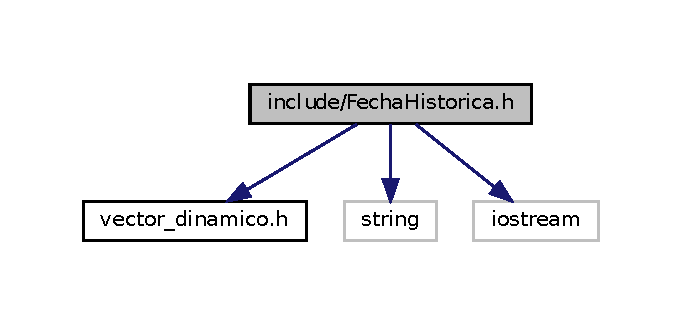
\includegraphics[width=328pt]{FechaHistorica_8h__incl}
\end{center}
\end{figure}
Gráfico de los archivos que directa o indirectamente incluyen a este archivo\+:\nopagebreak
\begin{figure}[H]
\begin{center}
\leavevmode
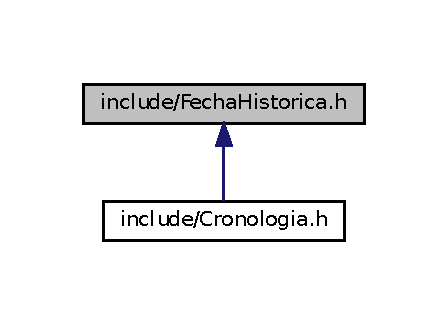
\includegraphics[width=215pt]{FechaHistorica_8h__dep__incl}
\end{center}
\end{figure}
\subsection*{Clases}
\begin{DoxyCompactItemize}
\item 
class \hyperlink{classFechaHistorica}{Fecha\+Historica}
\begin{DoxyCompactList}\small\item\em T.\+D.\+A. Fecha Historica. \end{DoxyCompactList}\end{DoxyCompactItemize}


\subsection{Descripción detallada}
Fichero cabecera del T\+DA \hyperlink{classFechaHistorica}{Fecha\+Historica}. 


%--- End generated contents ---

% Index
\backmatter
\newpage
\phantomsection
\clearemptydoublepage
\addcontentsline{toc}{chapter}{Índice}
\printindex

\end{document}
